\documentclass[1p]{elsarticle_modified}
%\bibliographystyle{elsarticle-num}

%\usepackage[colorlinks]{hyperref}
%\usepackage{abbrmath_seonhwa} %\Abb, \Ascr, \Acal ,\Abf, \Afrak
\usepackage{amsfonts}
\usepackage{amssymb}
\usepackage{amsmath}
\usepackage{amsthm}
\usepackage{scalefnt}
\usepackage{amsbsy}
\usepackage{kotex}
\usepackage{caption}
\usepackage{subfig}
\usepackage{color}
\usepackage{graphicx}
\usepackage{xcolor} %% white, black, red, green, blue, cyan, magenta, yellow
\usepackage{float}
\usepackage{setspace}
\usepackage{hyperref}

\usepackage{tikz}
\usetikzlibrary{arrows}

\usepackage{multirow}
\usepackage{array} % fixed length table
\usepackage{hhline}

%%%%%%%%%%%%%%%%%%%%%
\makeatletter
\renewcommand*\env@matrix[1][\arraystretch]{%
	\edef\arraystretch{#1}%
	\hskip -\arraycolsep
	\let\@ifnextchar\new@ifnextchar
	\array{*\c@MaxMatrixCols c}}
\makeatother %https://tex.stackexchange.com/questions/14071/how-can-i-increase-the-line-spacing-in-a-matrix
%%%%%%%%%%%%%%%

\usepackage[normalem]{ulem}

\newcommand{\msout}[1]{\ifmmode\text{\sout{\ensuremath{#1}}}\else\sout{#1}\fi}
%SOURCE: \msout is \stkout macro in https://tex.stackexchange.com/questions/20609/strikeout-in-math-mode

\newcommand{\cancel}[1]{
	\ifmmode
	{\color{red}\msout{#1}}
	\else
	{\color{red}\sout{#1}}
	\fi
}

\newcommand{\add}[1]{
	{\color{blue}\uwave{#1}}
}

\newcommand{\replace}[2]{
	\ifmmode
	{\color{red}\msout{#1}}{\color{blue}\uwave{#2}}
	\else
	{\color{red}\sout{#1}}{\color{blue}\uwave{#2}}
	\fi
}

\newcommand{\Sol}{\mathcal{S}} %segment
\newcommand{\D}{D} %diagram
\newcommand{\A}{\mathcal{A}} %arc


%%%%%%%%%%%%%%%%%%%%%%%%%%%%%5 test

\def\sl{\operatorname{\textup{SL}}(2,\Cbb)}
\def\psl{\operatorname{\textup{PSL}}(2,\Cbb)}
\def\quan{\mkern 1mu \triangleright \mkern 1mu}

\theoremstyle{definition}
\newtheorem{thm}{Theorem}[section]
\newtheorem{prop}[thm]{Proposition}
\newtheorem{lem}[thm]{Lemma}
\newtheorem{ques}[thm]{Question}
\newtheorem{cor}[thm]{Corollary}
\newtheorem{defn}[thm]{Definition}
\newtheorem{exam}[thm]{Example}
\newtheorem{rmk}[thm]{Remark}
\newtheorem{alg}[thm]{Algorithm}

\newcommand{\I}{\sqrt{-1}}
\begin{document}

%\begin{frontmatter}
%
%\title{Boundary parabolic representations of knots up to 8 crossings}
%
%%% Group authors per affiliation:
%\author{Yunhi Cho} 
%\address{Department of Mathematics, University of Seoul, Seoul, Korea}
%\ead{yhcho@uos.ac.kr}
%
%
%\author{Seonhwa Kim} %\fnref{s_kim}}
%\address{Center for Geometry and Physics, Institute for Basic Science, Pohang, 37673, Korea}
%\ead{ryeona17@ibs.re.kr}
%
%\author{Hyuk Kim}
%\address{Department of Mathematical Sciences, Seoul National University, Seoul 08826, Korea}
%\ead{hyukkim@snu.ac.kr}
%
%\author{Seokbeom Yoon}
%\address{Department of Mathematical Sciences, Seoul National University, Seoul, 08826,  Korea}
%\ead{sbyoon15@snu.ac.kr}
%
%\begin{abstract}
%We find all boundary parabolic representation of knots up to 8 crossings.
%
%\end{abstract}
%\begin{keyword}
%    \MSC[2010] 57M25 
%\end{keyword}
%
%\end{frontmatter}

%\linenumbers
%\tableofcontents
%
\newcommand\colored[1]{\textcolor{white}{\rule[-0.35ex]{0.8em}{1.4ex}}\kern-0.8em\color{red} #1}%
%\newcommand\colored[1]{\textcolor{white}{ #1}\kern-2.17ex	\textcolor{white}{ #1}\kern-1.81ex	\textcolor{white}{ #1}\kern-2.15ex\color{red}#1	}

{\Large $\underline{12a_{1049}~(K12a_{1049})}$}

\setlength{\tabcolsep}{10pt}
\renewcommand{\arraystretch}{1.6}
\vspace{1cm}\begin{tabular}{m{100pt}>{\centering\arraybackslash}m{274pt}}
\multirow{5}{120pt}{
	\centering
	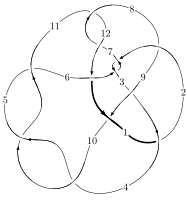
\includegraphics[width=112pt]{../../../GIT/diagram.site/Diagrams/png/1850_12a_1049.png}\\
\ \ \ A knot diagram\footnotemark}&
\allowdisplaybreaks
\textbf{Linearized knot diagam} \\
\cline{2-2}
 &
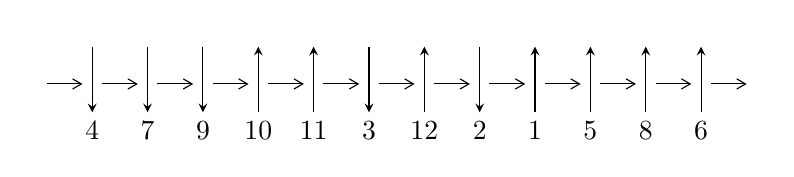
\begin{tikzpicture}[x=20pt, y=17pt]
	% nodes
	\node (C0) at (0, 0) {};
	\node (C1) at (1, 0) {};
	\node (C1U) at (1, +1) {};
	\node (C1D) at (1, -1) {4};

	\node (C2) at (2, 0) {};
	\node (C2U) at (2, +1) {};
	\node (C2D) at (2, -1) {7};

	\node (C3) at (3, 0) {};
	\node (C3U) at (3, +1) {};
	\node (C3D) at (3, -1) {9};

	\node (C4) at (4, 0) {};
	\node (C4U) at (4, +1) {};
	\node (C4D) at (4, -1) {10};

	\node (C5) at (5, 0) {};
	\node (C5U) at (5, +1) {};
	\node (C5D) at (5, -1) {11};

	\node (C6) at (6, 0) {};
	\node (C6U) at (6, +1) {};
	\node (C6D) at (6, -1) {3};

	\node (C7) at (7, 0) {};
	\node (C7U) at (7, +1) {};
	\node (C7D) at (7, -1) {12};

	\node (C8) at (8, 0) {};
	\node (C8U) at (8, +1) {};
	\node (C8D) at (8, -1) {2};

	\node (C9) at (9, 0) {};
	\node (C9U) at (9, +1) {};
	\node (C9D) at (9, -1) {1};

	\node (C10) at (10, 0) {};
	\node (C10U) at (10, +1) {};
	\node (C10D) at (10, -1) {5};

	\node (C11) at (11, 0) {};
	\node (C11U) at (11, +1) {};
	\node (C11D) at (11, -1) {8};

	\node (C12) at (12, 0) {};
	\node (C12U) at (12, +1) {};
	\node (C12D) at (12, -1) {6};
	\node (C13) at (13, 0) {};

	% arrows
	\draw[->,>={angle 60}]
	(C0) edge (C1) (C1) edge (C2) (C2) edge (C3) (C3) edge (C4) (C4) edge (C5) (C5) edge (C6) (C6) edge (C7) (C7) edge (C8) (C8) edge (C9) (C9) edge (C10) (C10) edge (C11) (C11) edge (C12) (C12) edge (C13) ;	\draw[->,>=stealth]
	(C1U) edge (C1D) (C2U) edge (C2D) (C3U) edge (C3D) (C4D) edge (C4U) (C5D) edge (C5U) (C6U) edge (C6D) (C7D) edge (C7U) (C8U) edge (C8D) (C9D) edge (C9U) (C10D) edge (C10U) (C11D) edge (C11U) (C12D) edge (C12U) ;
	\end{tikzpicture} \\
\hhline{~~} \\& 
\textbf{Solving Sequence} \\ \cline{2-2} 
 &
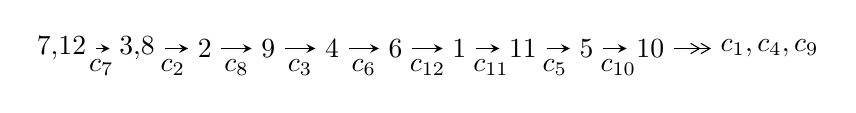
\begin{tikzpicture}[x=23pt, y=7pt]
	% node
	\node (A0) at (-1/8, 0) {7,12};
	\node (A1) at (17/16, 0) {3,8};
	\node (A2) at (17/8, 0) {2};
	\node (A3) at (25/8, 0) {9};
	\node (A4) at (33/8, 0) {4};
	\node (A5) at (41/8, 0) {6};
	\node (A6) at (49/8, 0) {1};
	\node (A7) at (57/8, 0) {11};
	\node (A8) at (65/8, 0) {5};
	\node (A9) at (73/8, 0) {10};
	\node (C1) at (1/2, -1) {$c_{7}$};
	\node (C2) at (13/8, -1) {$c_{2}$};
	\node (C3) at (21/8, -1) {$c_{8}$};
	\node (C4) at (29/8, -1) {$c_{3}$};
	\node (C5) at (37/8, -1) {$c_{6}$};
	\node (C6) at (45/8, -1) {$c_{12}$};
	\node (C7) at (53/8, -1) {$c_{11}$};
	\node (C8) at (61/8, -1) {$c_{5}$};
	\node (C9) at (69/8, -1) {$c_{10}$};
	\node (A10) at (11, 0) {$c_{1},c_{4},c_{9}$};

	% edge
	\draw[->,>=stealth]	
	(A0) edge (A1) (A1) edge (A2) (A2) edge (A3) (A3) edge (A4) (A4) edge (A5) (A5) edge (A6) (A6) edge (A7) (A7) edge (A8) (A8) edge (A9) ;
	\draw[->>,>={angle 60}]	
	(A9) edge (A10);
\end{tikzpicture} \\ 

\end{tabular} \\

\footnotetext{
The image of knot diagram is generated by the software ``\textbf{Draw programme}" developed by Andrew Bartholomew(\url{http://www.layer8.co.uk/maths/draw/index.htm\#Running-draw}), where we modified some parts for our purpose(\url{https://github.com/CATsTAILs/LinksPainter}).
}\phantom \\ \newline 
\centering \textbf{Ideals for irreducible components\footnotemark of $X_{\text{par}}$} 
 
\begin{align*}
I^u_{1}&=\langle 
3.93920\times10^{654} u^{144}-5.11511\times10^{654} u^{143}+\cdots+4.99948\times10^{655} b-1.30043\times10^{657},\\
\phantom{I^u_{1}}&\phantom{= \langle  }6.67458\times10^{656} u^{144}-2.62279\times10^{657} u^{143}+\cdots+2.63273\times10^{659} a-2.78924\times10^{661},\\
\phantom{I^u_{1}}&\phantom{= \langle  }u^{145}- u^{144}+\cdots-16062 u+2633\rangle \\
I^u_{2}&=\langle 
-362172324953570 u^{37}-2982250257830 u^{36}+\cdots+72532752090989 b-1020843727622321,\\
\phantom{I^u_{2}}&\phantom{= \langle  }1.47266\times10^{18} u^{37}-5.12596\times10^{17} u^{36}+\cdots+1.04955\times10^{17} a+1.03174\times10^{19},\;u^{38}-2 u^{37}+\cdots-2 u+1\rangle \\
\\
\end{align*}
\raggedright * 2 irreducible components of $\dim_{\mathbb{C}}=0$, with total 183 representations.\\
\footnotetext{All coefficients of polynomials are rational numbers. But the coefficients are sometimes approximated in decimal forms when there is not enough margin.}
\newpage
\renewcommand{\arraystretch}{1}
\centering \section*{I. $I^u_{1}= \langle 3.94\times10^{654} u^{144}-5.12\times10^{654} u^{143}+\cdots+5.00\times10^{655} b-1.30\times10^{657},\;6.67\times10^{656} u^{144}-2.62\times10^{657} u^{143}+\cdots+2.63\times10^{659} a-2.79\times10^{661},\;u^{145}- u^{144}+\cdots-16062 u+2633 \rangle$}
\flushleft \textbf{(i) Arc colorings}\\
\begin{tabular}{m{7pt} m{180pt} m{7pt} m{180pt} }
\flushright $a_{7}=$&$\begin{pmatrix}1\\0\end{pmatrix}$ \\
\flushright $a_{12}=$&$\begin{pmatrix}0\\u\end{pmatrix}$ \\
\flushright $a_{3}=$&$\begin{pmatrix}-0.00253523 u^{144}+0.00996226 u^{143}+\cdots-687.422 u+105.945\\-0.0787922 u^{144}+0.102313 u^{143}+\cdots-394.382 u+26.0113\end{pmatrix}$ \\
\flushright $a_{8}=$&$\begin{pmatrix}1\\- u^2\end{pmatrix}$ \\
\flushright $a_{2}=$&$\begin{pmatrix}-0.0813275 u^{144}+0.112275 u^{143}+\cdots-1081.80 u+131.956\\-0.0787922 u^{144}+0.102313 u^{143}+\cdots-394.382 u+26.0113\end{pmatrix}$ \\
\flushright $a_{9}=$&$\begin{pmatrix}-0.0156513 u^{144}+0.00321289 u^{143}+\cdots-1.16336 u+27.2456\\-0.0333935 u^{144}+0.0238342 u^{143}+\cdots+458.330 u-85.3090\end{pmatrix}$ \\
\flushright $a_{4}=$&$\begin{pmatrix}-0.0917059 u^{144}+0.0792602 u^{143}+\cdots-1383.07 u+97.5660\\-0.0653164 u^{144}+0.120138 u^{143}+\cdots-420.405 u+53.7737\end{pmatrix}$ \\
\flushright $a_{6}=$&$\begin{pmatrix}0.00702213 u^{144}-0.0568846 u^{143}+\cdots-131.329 u+23.4287\\-0.0346254 u^{144}-0.0368177 u^{143}+\cdots+1417.40 u-234.089\end{pmatrix}$ \\
\flushright $a_{1}=$&$\begin{pmatrix}-0.0542114 u^{144}+0.0364899 u^{143}+\cdots+666.046 u-67.6965\\-0.0683835 u^{144}+0.168362 u^{143}+\cdots-1380.22 u+183.560\end{pmatrix}$ \\
\flushright $a_{11}=$&$\begin{pmatrix}- u\\u^3+u\end{pmatrix}$ \\
\flushright $a_{5}=$&$\begin{pmatrix}-0.0269487 u^{144}-0.0728494 u^{143}+\cdots+881.150 u-149.718\\-0.0476591 u^{144}+0.00887131 u^{143}+\cdots+1117.54 u-192.423\end{pmatrix}$ \\
\flushright $a_{10}=$&$\begin{pmatrix}-0.0356556 u^{144}-0.00733218 u^{143}+\cdots+1458.74 u-297.707\\-0.0774097 u^{144}+0.0610850 u^{143}+\cdots+1344.70 u-235.204\end{pmatrix}$\\&\end{tabular}
\flushleft \textbf{(ii) Obstruction class $= -1$}\\~\\
\flushleft \textbf{(iii) Cusp Shapes $= -0.436067 u^{144}+0.275264 u^{143}+\cdots+7010.50 u-1340.34$}\\~\\
\newpage\renewcommand{\arraystretch}{1}
\flushleft \textbf{(iv) u-Polynomials at the component}\newline \\
\begin{tabular}{m{50pt}|m{274pt}}
Crossings & \hspace{64pt}u-Polynomials at each crossing \\
\hline $$\begin{aligned}c_{1}\end{aligned}$$&$\begin{aligned}
&u^{145}-11 u^{144}+\cdots-734954 u+73421
\end{aligned}$\\
\hline $$\begin{aligned}c_{2},c_{6}\end{aligned}$$&$\begin{aligned}
&u^{145}- u^{144}+\cdots-3830 u-803
\end{aligned}$\\
\hline $$\begin{aligned}c_{3}\end{aligned}$$&$\begin{aligned}
&u^{145}+u^{144}+\cdots-192 u-16
\end{aligned}$\\
\hline $$\begin{aligned}c_{4},c_{5},c_{10}\end{aligned}$$&$\begin{aligned}
&u^{145}- u^{144}+\cdots-58 u-3
\end{aligned}$\\
\hline $$\begin{aligned}c_{7},c_{11}\end{aligned}$$&$\begin{aligned}
&u^{145}+u^{144}+\cdots-16062 u-2633
\end{aligned}$\\
\hline $$\begin{aligned}c_{8}\end{aligned}$$&$\begin{aligned}
&u^{145}- u^{144}+\cdots-38691220 u-1160044
\end{aligned}$\\
\hline $$\begin{aligned}c_{9}\end{aligned}$$&$\begin{aligned}
&u^{145}-5 u^{144}+\cdots-62879 u+16999
\end{aligned}$\\
\hline $$\begin{aligned}c_{12}\end{aligned}$$&$\begin{aligned}
&u^{145}+u^{144}+\cdots+151613 u-160147
\end{aligned}$\\
\hline
\end{tabular}\\~\\
\newpage\renewcommand{\arraystretch}{1}
\flushleft \textbf{(v) Riley Polynomials at the component}\newline \\
\begin{tabular}{m{50pt}|m{274pt}}
Crossings & \hspace{64pt}Riley Polynomials at each crossing \\
\hline $$\begin{aligned}c_{1}\end{aligned}$$&$\begin{aligned}
&y^{145}+47 y^{144}+\cdots-203428626426 y-5390643241
\end{aligned}$\\
\hline $$\begin{aligned}c_{2},c_{6}\end{aligned}$$&$\begin{aligned}
&y^{145}+79 y^{144}+\cdots-29939356 y-644809
\end{aligned}$\\
\hline $$\begin{aligned}c_{3}\end{aligned}$$&$\begin{aligned}
&y^{145}-13 y^{144}+\cdots+15136 y-256
\end{aligned}$\\
\hline $$\begin{aligned}c_{4},c_{5},c_{10}\end{aligned}$$&$\begin{aligned}
&y^{145}-153 y^{144}+\cdots-50 y-9
\end{aligned}$\\
\hline $$\begin{aligned}c_{7},c_{11}\end{aligned}$$&$\begin{aligned}
&y^{145}+69 y^{144}+\cdots-222903276 y-6932689
\end{aligned}$\\
\hline $$\begin{aligned}c_{8}\end{aligned}$$&$\begin{aligned}
&y^{145}+25 y^{144}+\cdots+139705969316016 y-1345702081936
\end{aligned}$\\
\hline $$\begin{aligned}c_{9}\end{aligned}$$&$\begin{aligned}
&y^{145}-41 y^{144}+\cdots+9501766269 y-288966001
\end{aligned}$\\
\hline $$\begin{aligned}c_{12}\end{aligned}$$&$\begin{aligned}
&y^{145}-21 y^{144}+\cdots-603561410741 y-25647061609
\end{aligned}$\\
\hline
\end{tabular}\\~\\
\newpage\flushleft \textbf{(vi) Complex Volumes and Cusp Shapes}
$$\begin{array}{c|c|c}  
\text{Solutions to }I^u_{1}& \I (\text{vol} + \sqrt{-1}CS) & \text{Cusp shape}\\
 \hline 
\begin{aligned}
u &= -0.345803 + 0.954006 I \\
a &= \phantom{-}0.405855 - 0.158222 I \\
b &= \phantom{-}1.199700 - 0.554323 I\end{aligned}
 & -2.42257 - 2.18881 I & \phantom{-0.000000 } 0 \\ \hline\begin{aligned}
u &= -0.345803 - 0.954006 I \\
a &= \phantom{-}0.405855 + 0.158222 I \\
b &= \phantom{-}1.199700 + 0.554323 I\end{aligned}
 & -2.42257 + 2.18881 I & \phantom{-0.000000 } 0 \\ \hline\begin{aligned}
u &= -0.328025 + 0.927715 I \\
a &= -2.69856 + 0.12274 I \\
b &= -0.268401 - 1.175380 I\end{aligned}
 & \phantom{-}9.26433 - 6.68590 I & \phantom{-0.000000 } 0 \\ \hline\begin{aligned}
u &= -0.328025 - 0.927715 I \\
a &= -2.69856 - 0.12274 I \\
b &= -0.268401 + 1.175380 I\end{aligned}
 & \phantom{-}9.26433 + 6.68590 I & \phantom{-0.000000 } 0 \\ \hline\begin{aligned}
u &= \phantom{-}0.324152 + 0.977516 I \\
a &= \phantom{-}0.192792 + 0.548668 I \\
b &= \phantom{-}1.126410 + 0.338613 I\end{aligned}
 & -3.59244 + 1.03408 I & \phantom{-0.000000 } 0 \\ \hline\begin{aligned}
u &= \phantom{-}0.324152 - 0.977516 I \\
a &= \phantom{-}0.192792 - 0.548668 I \\
b &= \phantom{-}1.126410 - 0.338613 I\end{aligned}
 & -3.59244 - 1.03408 I & \phantom{-0.000000 } 0 \\ \hline\begin{aligned}
u &= -0.588801 + 0.763843 I \\
a &= \phantom{-}1.68959 - 1.03593 I \\
b &= \phantom{-}0.380153 + 1.264270 I\end{aligned}
 & \phantom{-}11.25430 + 3.12129 I & \phantom{-0.000000 } 0 \\ \hline\begin{aligned}
u &= -0.588801 - 0.763843 I \\
a &= \phantom{-}1.68959 + 1.03593 I \\
b &= \phantom{-}0.380153 - 1.264270 I\end{aligned}
 & \phantom{-}11.25430 - 3.12129 I & \phantom{-0.000000 } 0 \\ \hline\begin{aligned}
u &= -0.557369 + 0.883050 I \\
a &= -0.391018 + 1.270450 I \\
b &= \phantom{-}0.22442 - 1.53873 I\end{aligned}
 & \phantom{-}10.89490 - 7.65848 I & \phantom{-0.000000 } 0 \\ \hline\begin{aligned}
u &= -0.557369 - 0.883050 I \\
a &= -0.391018 - 1.270450 I \\
b &= \phantom{-}0.22442 + 1.53873 I\end{aligned}
 & \phantom{-}10.89490 + 7.65848 I & \phantom{-0.000000 } 0\\
 \hline 
 \end{array}$$\newpage$$\begin{array}{c|c|c}  
\text{Solutions to }I^u_{1}& \I (\text{vol} + \sqrt{-1}CS) & \text{Cusp shape}\\
 \hline 
\begin{aligned}
u &= -0.734129 + 0.604314 I \\
a &= \phantom{-}0.203457 - 0.892143 I \\
b &= -0.372220 + 1.070590 I\end{aligned}
 & \phantom{-}2.05754 - 0.26115 I & \phantom{-0.000000 } 0 \\ \hline\begin{aligned}
u &= -0.734129 - 0.604314 I \\
a &= \phantom{-}0.203457 + 0.892143 I \\
b &= -0.372220 - 1.070590 I\end{aligned}
 & \phantom{-}2.05754 + 0.26115 I & \phantom{-0.000000 } 0 \\ \hline\begin{aligned}
u &= -0.556442 + 0.895770 I \\
a &= -1.06457 + 1.12076 I \\
b &= -0.757358 - 1.022820 I\end{aligned}
 & \phantom{-}1.26728 - 4.74488 I & \phantom{-0.000000 } 0 \\ \hline\begin{aligned}
u &= -0.556442 - 0.895770 I \\
a &= -1.06457 - 1.12076 I \\
b &= -0.757358 + 1.022820 I\end{aligned}
 & \phantom{-}1.26728 + 4.74488 I & \phantom{-0.000000 } 0 \\ \hline\begin{aligned}
u &= \phantom{-}0.340241 + 1.002790 I \\
a &= -0.399127 + 0.016272 I \\
b &= \phantom{-}0.742111 + 0.658754 I\end{aligned}
 & -2.25285 - 0.78087 I & \phantom{-0.000000 } 0 \\ \hline\begin{aligned}
u &= \phantom{-}0.340241 - 1.002790 I \\
a &= -0.399127 - 0.016272 I \\
b &= \phantom{-}0.742111 - 0.658754 I\end{aligned}
 & -2.25285 + 0.78087 I & \phantom{-0.000000 } 0 \\ \hline\begin{aligned}
u &= -0.888985 + 0.297233 I \\
a &= -0.176531 - 1.010800 I \\
b &= \phantom{-}0.846576 + 0.135584 I\end{aligned}
 & \phantom{-}7.00493 + 7.38643 I & \phantom{-0.000000 } 0 \\ \hline\begin{aligned}
u &= -0.888985 - 0.297233 I \\
a &= -0.176531 + 1.010800 I \\
b &= \phantom{-}0.846576 - 0.135584 I\end{aligned}
 & \phantom{-}7.00493 - 7.38643 I & \phantom{-0.000000 } 0 \\ \hline\begin{aligned}
u &= -0.284744 + 0.878018 I \\
a &= \phantom{-}0.019213 + 0.567381 I \\
b &= -1.15865 + 0.85075 I\end{aligned}
 & \phantom{-}0.61703 + 2.26391 I & \phantom{-0.000000 } 0 \\ \hline\begin{aligned}
u &= -0.284744 - 0.878018 I \\
a &= \phantom{-}0.019213 - 0.567381 I \\
b &= -1.15865 - 0.85075 I\end{aligned}
 & \phantom{-}0.61703 - 2.26391 I & \phantom{-0.000000 } 0\\
 \hline 
 \end{array}$$\newpage$$\begin{array}{c|c|c}  
\text{Solutions to }I^u_{1}& \I (\text{vol} + \sqrt{-1}CS) & \text{Cusp shape}\\
 \hline 
\begin{aligned}
u &= \phantom{-}0.604047 + 0.901518 I \\
a &= \phantom{-}0.67281 + 1.57252 I \\
b &= \phantom{-}0.600521 - 0.752227 I\end{aligned}
 & -2.00786 + 4.37308 I & \phantom{-0.000000 } 0 \\ \hline\begin{aligned}
u &= \phantom{-}0.604047 - 0.901518 I \\
a &= \phantom{-}0.67281 - 1.57252 I \\
b &= \phantom{-}0.600521 + 0.752227 I\end{aligned}
 & -2.00786 - 4.37308 I & \phantom{-0.000000 } 0 \\ \hline\begin{aligned}
u &= -0.261266 + 0.871926 I \\
a &= \phantom{-}0.501018 - 0.072340 I \\
b &= \phantom{-}1.210590 - 0.073871 I\end{aligned}
 & -1.94634 - 0.41173 I & \phantom{-0.000000 } 0 \\ \hline\begin{aligned}
u &= -0.261266 - 0.871926 I \\
a &= \phantom{-}0.501018 + 0.072340 I \\
b &= \phantom{-}1.210590 + 0.073871 I\end{aligned}
 & -1.94634 + 0.41173 I & \phantom{-0.000000 } 0 \\ \hline\begin{aligned}
u &= -0.350231 + 0.838408 I \\
a &= \phantom{-}0.33774 - 2.26170 I \\
b &= -0.19744 + 1.45081 I\end{aligned}
 & \phantom{-}9.55110 + 3.78182 I & \phantom{-0.000000 } 0 \\ \hline\begin{aligned}
u &= -0.350231 - 0.838408 I \\
a &= \phantom{-}0.33774 + 2.26170 I \\
b &= -0.19744 - 1.45081 I\end{aligned}
 & \phantom{-}9.55110 - 3.78182 I & \phantom{-0.000000 } 0 \\ \hline\begin{aligned}
u &= \phantom{-}0.867409 + 0.664015 I \\
a &= \phantom{-}1.33358 + 1.18745 I \\
b &= \phantom{-}0.511867 - 0.916704 I\end{aligned}
 & \phantom{-}9.02544 + 4.66895 I & \phantom{-0.000000 } 0 \\ \hline\begin{aligned}
u &= \phantom{-}0.867409 - 0.664015 I \\
a &= \phantom{-}1.33358 - 1.18745 I \\
b &= \phantom{-}0.511867 + 0.916704 I\end{aligned}
 & \phantom{-}9.02544 - 4.66895 I & \phantom{-0.000000 } 0 \\ \hline\begin{aligned}
u &= \phantom{-}0.440100 + 1.006090 I \\
a &= -1.224450 - 0.325949 I \\
b &= -0.750553 + 1.077560 I\end{aligned}
 & \phantom{-}7.75099 + 3.57028 I & \phantom{-0.000000 } 0 \\ \hline\begin{aligned}
u &= \phantom{-}0.440100 - 1.006090 I \\
a &= -1.224450 + 0.325949 I \\
b &= -0.750553 - 1.077560 I\end{aligned}
 & \phantom{-}7.75099 - 3.57028 I & \phantom{-0.000000 } 0\\
 \hline 
 \end{array}$$\newpage$$\begin{array}{c|c|c}  
\text{Solutions to }I^u_{1}& \I (\text{vol} + \sqrt{-1}CS) & \text{Cusp shape}\\
 \hline 
\begin{aligned}
u &= \phantom{-}0.505174 + 0.975773 I \\
a &= -1.062970 - 0.821190 I \\
b &= -0.440321 + 1.236690 I\end{aligned}
 & \phantom{-}3.50637 + 0.15818 I & \phantom{-0.000000 } 0 \\ \hline\begin{aligned}
u &= \phantom{-}0.505174 - 0.975773 I \\
a &= -1.062970 + 0.821190 I \\
b &= -0.440321 - 1.236690 I\end{aligned}
 & \phantom{-}3.50637 - 0.15818 I & \phantom{-0.000000 } 0 \\ \hline\begin{aligned}
u &= -0.816047 + 0.351664 I \\
a &= \phantom{-}0.62662 - 1.97885 I \\
b &= -0.441672 + 1.272420 I\end{aligned}
 & \phantom{-}7.22642 + 4.50090 I & \phantom{-0.000000 } 0 \\ \hline\begin{aligned}
u &= -0.816047 - 0.351664 I \\
a &= \phantom{-}0.62662 + 1.97885 I \\
b &= -0.441672 - 1.272420 I\end{aligned}
 & \phantom{-}7.22642 - 4.50090 I & \phantom{-0.000000 } 0 \\ \hline\begin{aligned}
u &= \phantom{-}0.172003 + 0.868140 I \\
a &= \phantom{-}1.41511 + 1.61234 I \\
b &= \phantom{-}0.512901 - 1.028200 I\end{aligned}
 & -1.65149 + 2.70585 I & \phantom{-0.000000 } 0 \\ \hline\begin{aligned}
u &= \phantom{-}0.172003 - 0.868140 I \\
a &= \phantom{-}1.41511 - 1.61234 I \\
b &= \phantom{-}0.512901 + 1.028200 I\end{aligned}
 & -1.65149 - 2.70585 I & \phantom{-0.000000 } 0 \\ \hline\begin{aligned}
u &= \phantom{-}0.520176 + 0.987540 I \\
a &= \phantom{-}1.87632 + 0.28971 I \\
b &= -0.013147 - 0.914276 I\end{aligned}
 & \phantom{-}8.38341 + 2.22541 I & \phantom{-0.000000 } 0 \\ \hline\begin{aligned}
u &= \phantom{-}0.520176 - 0.987540 I \\
a &= \phantom{-}1.87632 - 0.28971 I \\
b &= -0.013147 + 0.914276 I\end{aligned}
 & \phantom{-}8.38341 - 2.22541 I & \phantom{-0.000000 } 0 \\ \hline\begin{aligned}
u &= -0.613687 + 0.955832 I \\
a &= -1.11690 + 1.01099 I \\
b &= -0.105898 - 0.657996 I\end{aligned}
 & -0.20713 - 2.36351 I & \phantom{-0.000000 } 0 \\ \hline\begin{aligned}
u &= -0.613687 - 0.955832 I \\
a &= -1.11690 - 1.01099 I \\
b &= -0.105898 + 0.657996 I\end{aligned}
 & -0.20713 + 2.36351 I & \phantom{-0.000000 } 0\\
 \hline 
 \end{array}$$\newpage$$\begin{array}{c|c|c}  
\text{Solutions to }I^u_{1}& \I (\text{vol} + \sqrt{-1}CS) & \text{Cusp shape}\\
 \hline 
\begin{aligned}
u &= \phantom{-}1.097380 + 0.301946 I \\
a &= \phantom{-}0.332759 + 1.297620 I \\
b &= -0.471455 - 1.199170 I\end{aligned}
 & \phantom{-}3.35249 - 8.83135 I & \phantom{-0.000000 } 0 \\ \hline\begin{aligned}
u &= \phantom{-}1.097380 - 0.301946 I \\
a &= \phantom{-}0.332759 - 1.297620 I \\
b &= -0.471455 + 1.199170 I\end{aligned}
 & \phantom{-}3.35249 + 8.83135 I & \phantom{-0.000000 } 0 \\ \hline\begin{aligned}
u &= \phantom{-}0.878396 + 0.726590 I \\
a &= \phantom{-}0.395276 - 0.928259 I \\
b &= \phantom{-}0.279022 + 1.012780 I\end{aligned}
 & \phantom{-}8.81024 + 1.64508 I & \phantom{-0.000000 } 0 \\ \hline\begin{aligned}
u &= \phantom{-}0.878396 - 0.726590 I \\
a &= \phantom{-}0.395276 + 0.928259 I \\
b &= \phantom{-}0.279022 - 1.012780 I\end{aligned}
 & \phantom{-}8.81024 - 1.64508 I & \phantom{-0.000000 } 0 \\ \hline\begin{aligned}
u &= -0.792951 + 0.819837 I \\
a &= -0.26165 + 1.84386 I \\
b &= -0.752024 - 0.886463 I\end{aligned}
 & \phantom{-}3.39079 - 5.74867 I & \phantom{-0.000000 } 0 \\ \hline\begin{aligned}
u &= -0.792951 - 0.819837 I \\
a &= -0.26165 - 1.84386 I \\
b &= -0.752024 + 0.886463 I\end{aligned}
 & \phantom{-}3.39079 + 5.74867 I & \phantom{-0.000000 } 0 \\ \hline\begin{aligned}
u &= \phantom{-}0.850767 + 0.116954 I \\
a &= \phantom{-}0.617587 + 0.606455 I \\
b &= \phantom{-}0.136051 + 0.150315 I\end{aligned}
 & \phantom{-}7.82911 + 1.59133 I & \phantom{-0.000000 } 0 \\ \hline\begin{aligned}
u &= \phantom{-}0.850767 - 0.116954 I \\
a &= \phantom{-}0.617587 - 0.606455 I \\
b &= \phantom{-}0.136051 - 0.150315 I\end{aligned}
 & \phantom{-}7.82911 - 1.59133 I & \phantom{-0.000000 } 0 \\ \hline\begin{aligned}
u &= -0.345604 + 1.091530 I \\
a &= -1.26749 + 1.72713 I \\
b &= -0.378450 - 1.032900 I\end{aligned}
 & -2.33621 - 5.74083 I & \phantom{-0.000000 } 0 \\ \hline\begin{aligned}
u &= -0.345604 - 1.091530 I \\
a &= -1.26749 - 1.72713 I \\
b &= -0.378450 + 1.032900 I\end{aligned}
 & -2.33621 + 5.74083 I & \phantom{-0.000000 } 0\\
 \hline 
 \end{array}$$\newpage$$\begin{array}{c|c|c}  
\text{Solutions to }I^u_{1}& \I (\text{vol} + \sqrt{-1}CS) & \text{Cusp shape}\\
 \hline 
\begin{aligned}
u &= -0.058524 + 1.144490 I \\
a &= \phantom{-}0.158625 + 0.369848 I \\
b &= \phantom{-}0.588702 + 0.442272 I\end{aligned}
 & -3.31707 - 1.65297 I & \phantom{-0.000000 } 0 \\ \hline\begin{aligned}
u &= -0.058524 - 1.144490 I \\
a &= \phantom{-}0.158625 - 0.369848 I \\
b &= \phantom{-}0.588702 - 0.442272 I\end{aligned}
 & -3.31707 + 1.65297 I & \phantom{-0.000000 } 0 \\ \hline\begin{aligned}
u &= \phantom{-}0.514670 + 0.679083 I \\
a &= \phantom{-}0.55502 - 1.91482 I \\
b &= -0.062270 + 1.239280 I\end{aligned}
 & \phantom{-}9.41329 + 2.00087 I & \phantom{-0.000000 } 0 \\ \hline\begin{aligned}
u &= \phantom{-}0.514670 - 0.679083 I \\
a &= \phantom{-}0.55502 + 1.91482 I \\
b &= -0.062270 - 1.239280 I\end{aligned}
 & \phantom{-}9.41329 - 2.00087 I & \phantom{-0.000000 } 0 \\ \hline\begin{aligned}
u &= -1.104570 + 0.365918 I \\
a &= -0.386339 + 1.298760 I \\
b &= \phantom{-}0.107291 - 1.129670 I\end{aligned}
 & \phantom{-}4.88864 - 0.23143 I & \phantom{-0.000000 } 0 \\ \hline\begin{aligned}
u &= -1.104570 - 0.365918 I \\
a &= -0.386339 - 1.298760 I \\
b &= \phantom{-}0.107291 + 1.129670 I\end{aligned}
 & \phantom{-}4.88864 + 0.23143 I & \phantom{-0.000000 } 0 \\ \hline\begin{aligned}
u &= -0.823066 + 0.076417 I \\
a &= -0.466418 + 1.242360 I \\
b &= \phantom{-}0.364043 - 1.223700 I\end{aligned}
 & \phantom{-}3.18766 + 4.05776 I & \phantom{-0.000000 } 0 \\ \hline\begin{aligned}
u &= -0.823066 - 0.076417 I \\
a &= -0.466418 - 1.242360 I \\
b &= \phantom{-}0.364043 + 1.223700 I\end{aligned}
 & \phantom{-}3.18766 - 4.05776 I & \phantom{-0.000000 } 0 \\ \hline\begin{aligned}
u &= \phantom{-}0.388068 + 1.107490 I \\
a &= -0.71969 - 1.40256 I \\
b &= -0.392541 + 0.823385 I\end{aligned}
 & -3.11646 - 1.04761 I & \phantom{-0.000000 } 0 \\ \hline\begin{aligned}
u &= \phantom{-}0.388068 - 1.107490 I \\
a &= -0.71969 + 1.40256 I \\
b &= -0.392541 - 0.823385 I\end{aligned}
 & -3.11646 + 1.04761 I & \phantom{-0.000000 } 0\\
 \hline 
 \end{array}$$\newpage$$\begin{array}{c|c|c}  
\text{Solutions to }I^u_{1}& \I (\text{vol} + \sqrt{-1}CS) & \text{Cusp shape}\\
 \hline 
\begin{aligned}
u &= -0.103494 + 1.176310 I \\
a &= -0.027478 - 0.268860 I \\
b &= -0.668246 + 0.907658 I\end{aligned}
 & \phantom{-}1.94861 + 1.75934 I & \phantom{-0.000000 } 0 \\ \hline\begin{aligned}
u &= -0.103494 - 1.176310 I \\
a &= -0.027478 + 0.268860 I \\
b &= -0.668246 - 0.907658 I\end{aligned}
 & \phantom{-}1.94861 - 1.75934 I & \phantom{-0.000000 } 0 \\ \hline\begin{aligned}
u &= -0.385175 + 1.120460 I \\
a &= -0.267590 + 0.748356 I \\
b &= -1.034940 - 0.199358 I\end{aligned}
 & \phantom{-}0.03735 - 3.82786 I & \phantom{-0.000000 } 0 \\ \hline\begin{aligned}
u &= -0.385175 - 1.120460 I \\
a &= -0.267590 - 0.748356 I \\
b &= -1.034940 + 0.199358 I\end{aligned}
 & \phantom{-}0.03735 + 3.82786 I & \phantom{-0.000000 } 0 \\ \hline\begin{aligned}
u &= -0.621640 + 1.016660 I \\
a &= \phantom{-}0.662878 - 0.166057 I \\
b &= -0.913543 + 0.603537 I\end{aligned}
 & \phantom{-}2.56176 + 0.24638 I & \phantom{-0.000000 } 0 \\ \hline\begin{aligned}
u &= -0.621640 - 1.016660 I \\
a &= \phantom{-}0.662878 + 0.166057 I \\
b &= -0.913543 - 0.603537 I\end{aligned}
 & \phantom{-}2.56176 - 0.24638 I & \phantom{-0.000000 } 0 \\ \hline\begin{aligned}
u &= \phantom{-}0.495869 + 1.084730 I \\
a &= -0.127005 - 0.065732 I \\
b &= -0.957253 + 0.085270 I\end{aligned}
 & \phantom{-}4.87201 + 5.66450 I & \phantom{-0.000000 } 0 \\ \hline\begin{aligned}
u &= \phantom{-}0.495869 - 1.084730 I \\
a &= -0.127005 + 0.065732 I \\
b &= -0.957253 - 0.085270 I\end{aligned}
 & \phantom{-}4.87201 - 5.66450 I & \phantom{-0.000000 } 0 \\ \hline\begin{aligned}
u &= \phantom{-}0.693662 + 0.407460 I \\
a &= -0.71838 - 1.41457 I \\
b &= \phantom{-}0.408383 + 1.171800 I\end{aligned}
 & \phantom{-}1.48479 - 2.67185 I & \phantom{-0.000000 } 0 \\ \hline\begin{aligned}
u &= \phantom{-}0.693662 - 0.407460 I \\
a &= -0.71838 + 1.41457 I \\
b &= \phantom{-}0.408383 - 1.171800 I\end{aligned}
 & \phantom{-}1.48479 + 2.67185 I & \phantom{-0.000000 } 0\\
 \hline 
 \end{array}$$\newpage$$\begin{array}{c|c|c}  
\text{Solutions to }I^u_{1}& \I (\text{vol} + \sqrt{-1}CS) & \text{Cusp shape}\\
 \hline 
\begin{aligned}
u &= -0.230026 + 0.767257 I \\
a &= -0.970699 + 0.672864 I \\
b &= -1.024820 - 0.662801 I\end{aligned}
 & \phantom{-}0.79432 - 4.66034 I & \phantom{-0.000000 } 0 \\ \hline\begin{aligned}
u &= -0.230026 - 0.767257 I \\
a &= -0.970699 - 0.672864 I \\
b &= -1.024820 + 0.662801 I\end{aligned}
 & \phantom{-}0.79432 + 4.66034 I & \phantom{-0.000000 } 0 \\ \hline\begin{aligned}
u &= \phantom{-}0.478404 + 1.100890 I \\
a &= -0.110896 - 0.242408 I \\
b &= -1.168450 - 0.365893 I\end{aligned}
 & -2.53806 + 8.45885 I & \phantom{-0.000000 } 0 \\ \hline\begin{aligned}
u &= \phantom{-}0.478404 - 1.100890 I \\
a &= -0.110896 + 0.242408 I \\
b &= -1.168450 + 0.365893 I\end{aligned}
 & -2.53806 - 8.45885 I & \phantom{-0.000000 } 0 \\ \hline\begin{aligned}
u &= -0.393115 + 1.134770 I \\
a &= -0.451919 + 0.056708 I \\
b &= -0.662117 + 0.337658 I\end{aligned}
 & -1.49516 - 2.91040 I & \phantom{-0.000000 } 0 \\ \hline\begin{aligned}
u &= -0.393115 - 1.134770 I \\
a &= -0.451919 - 0.056708 I \\
b &= -0.662117 - 0.337658 I\end{aligned}
 & -1.49516 + 2.91040 I & \phantom{-0.000000 } 0 \\ \hline\begin{aligned}
u &= \phantom{-}0.392411 + 1.142680 I \\
a &= \phantom{-}1.48660 + 0.54049 I \\
b &= \phantom{-}0.394496 - 1.133540 I\end{aligned}
 & \phantom{-}1.80870 + 6.32768 I & \phantom{-0.000000 } 0 \\ \hline\begin{aligned}
u &= \phantom{-}0.392411 - 1.142680 I \\
a &= \phantom{-}1.48660 - 0.54049 I \\
b &= \phantom{-}0.394496 + 1.133540 I\end{aligned}
 & \phantom{-}1.80870 - 6.32768 I & \phantom{-0.000000 } 0 \\ \hline\begin{aligned}
u &= -0.705793 + 0.990562 I \\
a &= \phantom{-}0.28312 - 1.65201 I \\
b &= \phantom{-}0.304649 + 0.976604 I\end{aligned}
 & -0.23839 - 3.04514 I & \phantom{-0.000000 } 0 \\ \hline\begin{aligned}
u &= -0.705793 - 0.990562 I \\
a &= \phantom{-}0.28312 + 1.65201 I \\
b &= \phantom{-}0.304649 - 0.976604 I\end{aligned}
 & -0.23839 + 3.04514 I & \phantom{-0.000000 } 0\\
 \hline 
 \end{array}$$\newpage$$\begin{array}{c|c|c}  
\text{Solutions to }I^u_{1}& \I (\text{vol} + \sqrt{-1}CS) & \text{Cusp shape}\\
 \hline 
\begin{aligned}
u &= \phantom{-}0.555300 + 1.087380 I \\
a &= \phantom{-}1.06919 + 1.35907 I \\
b &= \phantom{-}0.67238 - 1.28571 I\end{aligned}
 & -0.52019 + 7.48497 I & \phantom{-0.000000 } 0 \\ \hline\begin{aligned}
u &= \phantom{-}0.555300 - 1.087380 I \\
a &= \phantom{-}1.06919 - 1.35907 I \\
b &= \phantom{-}0.67238 + 1.28571 I\end{aligned}
 & -0.52019 - 7.48497 I & \phantom{-0.000000 } 0 \\ \hline\begin{aligned}
u &= \phantom{-}0.385611 + 0.675496 I \\
a &= -0.165168 + 0.873153 I \\
b &= -0.50627 - 1.42083 I\end{aligned}
 & \phantom{-}8.91007 - 0.02541 I & \phantom{-0.000000 } 0 \\ \hline\begin{aligned}
u &= \phantom{-}0.385611 - 0.675496 I \\
a &= -0.165168 - 0.873153 I \\
b &= -0.50627 + 1.42083 I\end{aligned}
 & \phantom{-}8.91007 + 0.02541 I & \phantom{-0.000000 } 0 \\ \hline\begin{aligned}
u &= \phantom{-}0.469606 + 0.565157 I \\
a &= \phantom{-}0.529296 + 1.185220 I \\
b &= -0.04133 - 1.46739 I\end{aligned}
 & \phantom{-}4.76124 + 3.98622 I & \phantom{-0.000000 } 0 \\ \hline\begin{aligned}
u &= \phantom{-}0.469606 - 0.565157 I \\
a &= \phantom{-}0.529296 - 1.185220 I \\
b &= -0.04133 + 1.46739 I\end{aligned}
 & \phantom{-}4.76124 - 3.98622 I & \phantom{-0.000000 } 0 \\ \hline\begin{aligned}
u &= -0.036072 + 0.729429 I \\
a &= \phantom{-}2.82162 - 0.62144 I \\
b &= \phantom{-}0.115132 + 0.590894 I\end{aligned}
 & -0.48013 + 3.62987 I & \phantom{-0.000000 } 0 \\ \hline\begin{aligned}
u &= -0.036072 - 0.729429 I \\
a &= \phantom{-}2.82162 + 0.62144 I \\
b &= \phantom{-}0.115132 - 0.590894 I\end{aligned}
 & -0.48013 - 3.62987 I & \phantom{-0.000000 } 0 \\ \hline\begin{aligned}
u &= -0.591497 + 1.129730 I \\
a &= -1.14298 + 1.62756 I \\
b &= -0.57681 - 1.41821 I\end{aligned}
 & \phantom{-}4.92365 - 9.73455 I & \phantom{-0.000000 } 0 \\ \hline\begin{aligned}
u &= -0.591497 - 1.129730 I \\
a &= -1.14298 - 1.62756 I \\
b &= -0.57681 + 1.41821 I\end{aligned}
 & \phantom{-}4.92365 + 9.73455 I & \phantom{-0.000000 } 0\\
 \hline 
 \end{array}$$\newpage$$\begin{array}{c|c|c}  
\text{Solutions to }I^u_{1}& \I (\text{vol} + \sqrt{-1}CS) & \text{Cusp shape}\\
 \hline 
\begin{aligned}
u &= -1.202830 + 0.456594 I \\
a &= -0.301957 + 1.347280 I \\
b &= \phantom{-}0.526033 - 1.214390 I\end{aligned}
 & \phantom{-}10.2118 + 12.4061 I & \phantom{-0.000000 } 0 \\ \hline\begin{aligned}
u &= -1.202830 - 0.456594 I \\
a &= -0.301957 - 1.347280 I \\
b &= \phantom{-}0.526033 + 1.214390 I\end{aligned}
 & \phantom{-}10.2118 - 12.4061 I & \phantom{-0.000000 } 0 \\ \hline\begin{aligned}
u &= \phantom{-}0.439555 + 1.213620 I \\
a &= \phantom{-}1.34068 + 1.84618 I \\
b &= \phantom{-}0.305634 - 1.064010 I\end{aligned}
 & \phantom{-}4.05655 + 8.00567 I & \phantom{-0.000000 } 0 \\ \hline\begin{aligned}
u &= \phantom{-}0.439555 - 1.213620 I \\
a &= \phantom{-}1.34068 - 1.84618 I \\
b &= \phantom{-}0.305634 + 1.064010 I\end{aligned}
 & \phantom{-}4.05655 - 8.00567 I & \phantom{-0.000000 } 0 \\ \hline\begin{aligned}
u &= -0.708359\phantom{ +0.000000I} \\
a &= \phantom{-}0.928437\phantom{ +0.000000I} \\
b &= -0.819861\phantom{ +0.000000I}\end{aligned}
 & \phantom{-}3.35565\phantom{ +0.000000I} & \phantom{-0.000000 } 0 \\ \hline\begin{aligned}
u &= -0.538987 + 1.194050 I \\
a &= \phantom{-}0.913305 - 0.910907 I \\
b &= \phantom{-}0.71204 + 1.24596 I\end{aligned}
 & \phantom{-}0.03098 - 9.00112 I & \phantom{-0.000000 } 0 \\ \hline\begin{aligned}
u &= -0.538987 - 1.194050 I \\
a &= \phantom{-}0.913305 + 0.910907 I \\
b &= \phantom{-}0.71204 - 1.24596 I\end{aligned}
 & \phantom{-}0.03098 + 9.00112 I & \phantom{-0.000000 } 0 \\ \hline\begin{aligned}
u &= -0.601955 + 1.165980 I \\
a &= -0.044068 - 0.317938 I \\
b &= \phantom{-}1.154840 - 0.281181 I\end{aligned}
 & \phantom{-}4.42380 - 12.82880 I & \phantom{-0.000000 } 0 \\ \hline\begin{aligned}
u &= -0.601955 - 1.165980 I \\
a &= -0.044068 + 0.317938 I \\
b &= \phantom{-}1.154840 + 0.281181 I\end{aligned}
 & \phantom{-}4.42380 + 12.82880 I & \phantom{-0.000000 } 0 \\ \hline\begin{aligned}
u &= -0.169508 + 1.304990 I \\
a &= -0.156883 + 0.369284 I \\
b &= -0.346648 + 0.528750 I\end{aligned}
 & -3.90414 - 2.47493 I & \phantom{-0.000000 } 0\\
 \hline 
 \end{array}$$\newpage$$\begin{array}{c|c|c}  
\text{Solutions to }I^u_{1}& \I (\text{vol} + \sqrt{-1}CS) & \text{Cusp shape}\\
 \hline 
\begin{aligned}
u &= -0.169508 - 1.304990 I \\
a &= -0.156883 - 0.369284 I \\
b &= -0.346648 - 0.528750 I\end{aligned}
 & -3.90414 + 2.47493 I & \phantom{-0.000000 } 0 \\ \hline\begin{aligned}
u &= -1.289440 + 0.280109 I \\
a &= -0.062415 - 1.325730 I \\
b &= -0.266590 + 0.977527 I\end{aligned}
 & \phantom{-}4.18624 + 0.94522 I & \phantom{-0.000000 } 0 \\ \hline\begin{aligned}
u &= -1.289440 - 0.280109 I \\
a &= -0.062415 + 1.325730 I \\
b &= -0.266590 - 0.977527 I\end{aligned}
 & \phantom{-}4.18624 - 0.94522 I & \phantom{-0.000000 } 0 \\ \hline\begin{aligned}
u &= -0.643415 + 1.171640 I \\
a &= \phantom{-}0.707992 - 1.121450 I \\
b &= \phantom{-}0.460605 + 1.275380 I\end{aligned}
 & \phantom{-}2.32392 - 5.81231 I & \phantom{-0.000000 } 0 \\ \hline\begin{aligned}
u &= -0.643415 - 1.171640 I \\
a &= \phantom{-}0.707992 + 1.121450 I \\
b &= \phantom{-}0.460605 - 1.275380 I\end{aligned}
 & \phantom{-}2.32392 + 5.81231 I & \phantom{-0.000000 } 0 \\ \hline\begin{aligned}
u &= -0.091486 + 1.381420 I \\
a &= \phantom{-}0.513358 - 0.822625 I \\
b &= \phantom{-}0.600974 + 0.683418 I\end{aligned}
 & \phantom{-}1.23433 + 3.68448 I & \phantom{-0.000000 } 0 \\ \hline\begin{aligned}
u &= -0.091486 - 1.381420 I \\
a &= \phantom{-}0.513358 + 0.822625 I \\
b &= \phantom{-}0.600974 - 0.683418 I\end{aligned}
 & \phantom{-}1.23433 - 3.68448 I & \phantom{-0.000000 } 0 \\ \hline\begin{aligned}
u &= \phantom{-}1.391550 + 0.047334 I \\
a &= \phantom{-}0.161483 - 1.138750 I \\
b &= \phantom{-}0.111054 + 0.710115 I\end{aligned}
 & \phantom{-}8.33476 - 1.74074 I & \phantom{-0.000000 } 0 \\ \hline\begin{aligned}
u &= \phantom{-}1.391550 - 0.047334 I \\
a &= \phantom{-}0.161483 + 1.138750 I \\
b &= \phantom{-}0.111054 - 0.710115 I\end{aligned}
 & \phantom{-}8.33476 + 1.74074 I & \phantom{-0.000000 } 0 \\ \hline\begin{aligned}
u &= \phantom{-}0.625069 + 1.245760 I \\
a &= \phantom{-}0.1407580 + 0.0100075 I \\
b &= \phantom{-}0.750814 + 0.328497 I\end{aligned}
 & \phantom{-}4.47210 + 3.99067 I & \phantom{-0.000000 } 0\\
 \hline 
 \end{array}$$\newpage$$\begin{array}{c|c|c}  
\text{Solutions to }I^u_{1}& \I (\text{vol} + \sqrt{-1}CS) & \text{Cusp shape}\\
 \hline 
\begin{aligned}
u &= \phantom{-}0.625069 - 1.245760 I \\
a &= \phantom{-}0.1407580 - 0.0100075 I \\
b &= \phantom{-}0.750814 - 0.328497 I\end{aligned}
 & \phantom{-}4.47210 - 3.99067 I & \phantom{-0.000000 } 0 \\ \hline\begin{aligned}
u &= \phantom{-}0.222261 + 0.561021 I \\
a &= -2.20669 - 0.58949 I \\
b &= -0.629023 - 0.819056 I\end{aligned}
 & \phantom{-}7.05607 - 2.06302 I & \phantom{-}4.89158 + 2.47548 I \\ \hline\begin{aligned}
u &= \phantom{-}0.222261 - 0.561021 I \\
a &= -2.20669 + 0.58949 I \\
b &= -0.629023 + 0.819056 I\end{aligned}
 & \phantom{-}7.05607 + 2.06302 I & \phantom{-}4.89158 - 2.47548 I \\ \hline\begin{aligned}
u &= \phantom{-}1.215480 + 0.699480 I \\
a &= \phantom{-}0.467435 + 1.232210 I \\
b &= -0.296032 - 1.110470 I\end{aligned}
 & \phantom{-}10.74500 - 3.42747 I & \phantom{-0.000000 } 0 \\ \hline\begin{aligned}
u &= \phantom{-}1.215480 - 0.699480 I \\
a &= \phantom{-}0.467435 - 1.232210 I \\
b &= -0.296032 + 1.110470 I\end{aligned}
 & \phantom{-}10.74500 + 3.42747 I & \phantom{-0.000000 } 0 \\ \hline\begin{aligned}
u &= \phantom{-}0.647896 + 1.246130 I \\
a &= -0.90290 - 1.18174 I \\
b &= -0.68168 + 1.27194 I\end{aligned}
 & \phantom{-}0.3866 + 15.0092 I & \phantom{-0.000000 } 0 \\ \hline\begin{aligned}
u &= \phantom{-}0.647896 - 1.246130 I \\
a &= -0.90290 + 1.18174 I \\
b &= -0.68168 - 1.27194 I\end{aligned}
 & \phantom{-}0.3866 - 15.0092 I & \phantom{-0.000000 } 0 \\ \hline\begin{aligned}
u &= \phantom{-}0.33818 + 1.39086 I \\
a &= \phantom{-}0.269297 + 0.393801 I \\
b &= \phantom{-}0.270102 + 0.633118 I\end{aligned}
 & \phantom{-}2.54991 + 5.38075 I & \phantom{-0.000000 } 0 \\ \hline\begin{aligned}
u &= \phantom{-}0.33818 - 1.39086 I \\
a &= \phantom{-}0.269297 - 0.393801 I \\
b &= \phantom{-}0.270102 - 0.633118 I\end{aligned}
 & \phantom{-}2.54991 - 5.38075 I & \phantom{-0.000000 } 0 \\ \hline\begin{aligned}
u &= \phantom{-}0.80176 + 1.18603 I \\
a &= -0.65389 - 1.37682 I \\
b &= -0.476159 + 1.274310 I\end{aligned}
 & \phantom{-}8.95941 + 10.59710 I & \phantom{-0.000000 } 0\\
 \hline 
 \end{array}$$\newpage$$\begin{array}{c|c|c}  
\text{Solutions to }I^u_{1}& \I (\text{vol} + \sqrt{-1}CS) & \text{Cusp shape}\\
 \hline 
\begin{aligned}
u &= \phantom{-}0.80176 - 1.18603 I \\
a &= -0.65389 + 1.37682 I \\
b &= -0.476159 - 1.274310 I\end{aligned}
 & \phantom{-}8.95941 - 10.59710 I & \phantom{-0.000000 } 0 \\ \hline\begin{aligned}
u &= \phantom{-}0.092808 + 0.553424 I \\
a &= -5.71826 - 1.96761 I \\
b &= -0.024806 + 0.712561 I\end{aligned}
 & \phantom{-}7.07374 - 5.24790 I & \phantom{-}5.63019 - 3.54213 I \\ \hline\begin{aligned}
u &= \phantom{-}0.092808 - 0.553424 I \\
a &= -5.71826 + 1.96761 I \\
b &= -0.024806 - 0.712561 I\end{aligned}
 & \phantom{-}7.07374 + 5.24790 I & \phantom{-}5.63019 + 3.54213 I \\ \hline\begin{aligned}
u &= \phantom{-}0.212048 + 0.506310 I \\
a &= -0.31682 - 2.46535 I \\
b &= \phantom{-}0.188620 + 1.374690 I\end{aligned}
 & \phantom{-}4.12511 - 3.28456 I & \phantom{-}16.4715 - 6.7726 I \\ \hline\begin{aligned}
u &= \phantom{-}0.212048 - 0.506310 I \\
a &= -0.31682 + 2.46535 I \\
b &= \phantom{-}0.188620 - 1.374690 I\end{aligned}
 & \phantom{-}4.12511 + 3.28456 I & \phantom{-}16.4715 + 6.7726 I \\ \hline\begin{aligned}
u &= -0.65741 + 1.29533 I \\
a &= -0.95566 + 1.06162 I \\
b &= -0.535496 - 1.111750 I\end{aligned}
 & \phantom{-}0.76477 - 7.58284 I & \phantom{-0.000000 } 0 \\ \hline\begin{aligned}
u &= -0.65741 - 1.29533 I \\
a &= -0.95566 - 1.06162 I \\
b &= -0.535496 + 1.111750 I\end{aligned}
 & \phantom{-}0.76477 + 7.58284 I & \phantom{-0.000000 } 0 \\ \hline\begin{aligned}
u &= \phantom{-}0.523584 + 0.152822 I \\
a &= -0.18200 - 1.59445 I \\
b &= -0.727053 - 0.007259 I\end{aligned}
 & -0.03447 - 4.40157 I & \phantom{-}3.14700 + 5.85331 I \\ \hline\begin{aligned}
u &= \phantom{-}0.523584 - 0.152822 I \\
a &= -0.18200 + 1.59445 I \\
b &= -0.727053 + 0.007259 I\end{aligned}
 & -0.03447 + 4.40157 I & \phantom{-}3.14700 - 5.85331 I \\ \hline\begin{aligned}
u &= -0.73675 + 1.25432 I \\
a &= \phantom{-}0.92669 - 1.36132 I \\
b &= \phantom{-}0.66085 + 1.29215 I\end{aligned}
 & \phantom{-}7.6185 - 19.2555 I & \phantom{-0.000000 } 0\\
 \hline 
 \end{array}$$\newpage$$\begin{array}{c|c|c}  
\text{Solutions to }I^u_{1}& \I (\text{vol} + \sqrt{-1}CS) & \text{Cusp shape}\\
 \hline 
\begin{aligned}
u &= -0.73675 - 1.25432 I \\
a &= \phantom{-}0.92669 + 1.36132 I \\
b &= \phantom{-}0.66085 - 1.29215 I\end{aligned}
 & \phantom{-}7.6185 + 19.2555 I & \phantom{-0.000000 } 0 \\ \hline\begin{aligned}
u &= -0.480237 + 0.234582 I \\
a &= -0.375118 - 0.018821 I \\
b &= -0.295874 + 0.287064 I\end{aligned}
 & \phantom{-}1.021370 - 0.466038 I & \phantom{-}8.14171 + 1.88483 I \\ \hline\begin{aligned}
u &= -0.480237 - 0.234582 I \\
a &= -0.375118 + 0.018821 I \\
b &= -0.295874 - 0.287064 I\end{aligned}
 & \phantom{-}1.021370 + 0.466038 I & \phantom{-}8.14171 - 1.88483 I \\ \hline\begin{aligned}
u &= -0.43867 + 1.41165 I \\
a &= -0.450257 + 0.204236 I \\
b &= \phantom{-}0.168962 - 0.809336 I\end{aligned}
 & -1.099940 - 0.850315 I & \phantom{-0.000000 } 0 \\ \hline\begin{aligned}
u &= -0.43867 - 1.41165 I \\
a &= -0.450257 - 0.204236 I \\
b &= \phantom{-}0.168962 + 0.809336 I\end{aligned}
 & -1.099940 + 0.850315 I & \phantom{-0.000000 } 0 \\ \hline\begin{aligned}
u &= \phantom{-}0.11903 + 1.49702 I \\
a &= -0.026180 + 0.143171 I \\
b &= -0.305262 - 0.805600 I\end{aligned}
 & -3.31162 - 4.19271 I & \phantom{-0.000000 } 0 \\ \hline\begin{aligned}
u &= \phantom{-}0.11903 - 1.49702 I \\
a &= -0.026180 - 0.143171 I \\
b &= -0.305262 + 0.805600 I\end{aligned}
 & -3.31162 + 4.19271 I & \phantom{-0.000000 } 0 \\ \hline\begin{aligned}
u &= \phantom{-}1.43342 + 0.46967 I \\
a &= -0.029346 - 1.364290 I \\
b &= \phantom{-}0.386152 + 1.009200 I\end{aligned}
 & \phantom{-}9.80632 - 0.98006 I & \phantom{-0.000000 } 0 \\ \hline\begin{aligned}
u &= \phantom{-}1.43342 - 0.46967 I \\
a &= -0.029346 + 1.364290 I \\
b &= \phantom{-}0.386152 - 1.009200 I\end{aligned}
 & \phantom{-}9.80632 + 0.98006 I & \phantom{-0.000000 } 0 \\ \hline\begin{aligned}
u &= \phantom{-}0.12757 + 1.56326 I \\
a &= \phantom{-}0.323689 + 0.383358 I \\
b &= \phantom{-}0.460855 - 0.875376 I\end{aligned}
 & \phantom{-}1.78418 + 7.91629 I & \phantom{-0.000000 } 0\\
 \hline 
 \end{array}$$\newpage$$\begin{array}{c|c|c}  
\text{Solutions to }I^u_{1}& \I (\text{vol} + \sqrt{-1}CS) & \text{Cusp shape}\\
 \hline 
\begin{aligned}
u &= \phantom{-}0.12757 - 1.56326 I \\
a &= \phantom{-}0.323689 - 0.383358 I \\
b &= \phantom{-}0.460855 + 0.875376 I\end{aligned}
 & \phantom{-}1.78418 - 7.91629 I & \phantom{-0.000000 } 0 \\ \hline\begin{aligned}
u &= \phantom{-}0.83963 + 1.36765 I \\
a &= \phantom{-}0.83266 + 1.24337 I \\
b &= \phantom{-}0.553484 - 1.117410 I\end{aligned}
 & \phantom{-}6.78833 + 8.90117 I & \phantom{-0.000000 } 0 \\ \hline\begin{aligned}
u &= \phantom{-}0.83963 - 1.36765 I \\
a &= \phantom{-}0.83266 - 1.24337 I \\
b &= \phantom{-}0.553484 + 1.117410 I\end{aligned}
 & \phantom{-}6.78833 - 8.90117 I & \phantom{-0.000000 } 0 \\ \hline\begin{aligned}
u &= \phantom{-}0.218657 + 0.169963 I \\
a &= -1.77650 - 0.96773 I \\
b &= \phantom{-}0.574300 + 0.265634 I\end{aligned}
 & -1.17962 - 0.99556 I & -2.00169 + 1.52521 I \\ \hline\begin{aligned}
u &= \phantom{-}0.218657 - 0.169963 I \\
a &= -1.77650 + 0.96773 I \\
b &= \phantom{-}0.574300 - 0.265634 I\end{aligned}
 & -1.17962 + 0.99556 I & -2.00169 - 1.52521 I\\
 \hline 
 \end{array}$$\newpage\newpage\renewcommand{\arraystretch}{1}
\centering \section*{II. $I^u_{2}= \langle -3.62\times10^{14} u^{37}-2.98\times10^{12} u^{36}+\cdots+7.25\times10^{13} b-1.02\times10^{15},\;1.47\times10^{18} u^{37}-5.13\times10^{17} u^{36}+\cdots+1.05\times10^{17} a+1.03\times10^{19},\;u^{38}-2 u^{37}+\cdots-2 u+1 \rangle$}
\flushleft \textbf{(i) Arc colorings}\\
\begin{tabular}{m{7pt} m{180pt} m{7pt} m{180pt} }
\flushright $a_{7}=$&$\begin{pmatrix}1\\0\end{pmatrix}$ \\
\flushright $a_{12}=$&$\begin{pmatrix}0\\u\end{pmatrix}$ \\
\flushright $a_{3}=$&$\begin{pmatrix}-14.0313 u^{37}+4.88397 u^{36}+\cdots+146.753 u-98.3034\\4.99322 u^{37}+0.0411159 u^{36}+\cdots-19.0974 u+14.0742\end{pmatrix}$ \\
\flushright $a_{8}=$&$\begin{pmatrix}1\\- u^2\end{pmatrix}$ \\
\flushright $a_{2}=$&$\begin{pmatrix}-9.03812 u^{37}+4.92508 u^{36}+\cdots+127.656 u-84.2292\\4.99322 u^{37}+0.0411159 u^{36}+\cdots-19.0974 u+14.0742\end{pmatrix}$ \\
\flushright $a_{9}=$&$\begin{pmatrix}-75.6584 u^{37}+152.041 u^{36}+\cdots-218.571 u-32.1504\\19.8361 u^{37}-48.6777 u^{36}+\cdots+72.7011 u-11.7856\end{pmatrix}$ \\
\flushright $a_{4}=$&$\begin{pmatrix}-20.5906 u^{37}+23.6730 u^{36}+\cdots-102.447 u-20.7979\\-15.9100 u^{37}+15.6491 u^{36}+\cdots+97.5284 u-64.4548\end{pmatrix}$ \\
\flushright $a_{6}=$&$\begin{pmatrix}37.0556 u^{37}-79.9036 u^{36}+\cdots+176.543 u-1.83582\\-11.9502 u^{37}+26.6200 u^{36}+\cdots-41.4503 u+8.71292\end{pmatrix}$ \\
\flushright $a_{1}=$&$\begin{pmatrix}-66.0396 u^{37}+168.125 u^{36}+\cdots-649.821 u+176.744\\-14.3942 u^{37}-4.49476 u^{36}+\cdots+166.779 u-101.848\end{pmatrix}$ \\
\flushright $a_{11}=$&$\begin{pmatrix}- u\\u^3+u\end{pmatrix}$ \\
\flushright $a_{5}=$&$\begin{pmatrix}38.4744 u^{37}-83.0531 u^{36}+\cdots+181.446 u+3.36074\\-10.5323 u^{37}+24.2087 u^{36}+\cdots-44.3115 u+3.20447\end{pmatrix}$ \\
\flushright $a_{10}=$&$\begin{pmatrix}77.5254 u^{37}-157.111 u^{36}+\cdots+400.913 u-46.7830\\-22.5221 u^{37}+43.4874 u^{36}+\cdots-120.877 u+30.7000\end{pmatrix}$\\&\end{tabular}
\flushleft \textbf{(ii) Obstruction class $= 1$}\\~\\
\flushleft \textbf{(iii) Cusp Shapes $= \frac{21354481039747811937}{104954892275661083} u^{37}-\frac{34594268770816226803}{104954892275661083} u^{36}+\cdots+\frac{46578911406556738133}{104954892275661083} u+\frac{17039115265124385250}{104954892275661083}$}\\~\\
\newpage\renewcommand{\arraystretch}{1}
\flushleft \textbf{(iv) u-Polynomials at the component}\newline \\
\begin{tabular}{m{50pt}|m{274pt}}
Crossings & \hspace{64pt}u-Polynomials at each crossing \\
\hline $$\begin{aligned}c_{1}\end{aligned}$$&$\begin{aligned}
&u^{38}-2 u^{37}+\cdots-2 u+1
\end{aligned}$\\
\hline $$\begin{aligned}c_{2}\end{aligned}$$&$\begin{aligned}
&u^{38}+2 u^{37}+\cdots+15 u^2+1
\end{aligned}$\\
\hline $$\begin{aligned}c_{3}\end{aligned}$$&$\begin{aligned}
&u^{38}-4 u^{36}+\cdots-5 u^2+1
\end{aligned}$\\
\hline $$\begin{aligned}c_{4},c_{5}\end{aligned}$$&$\begin{aligned}
&u^{38}-22 u^{36}+\cdots+14 u^2+1
\end{aligned}$\\
\hline $$\begin{aligned}c_{6}\end{aligned}$$&$\begin{aligned}
&u^{38}-2 u^{37}+\cdots+15 u^2+1
\end{aligned}$\\
\hline $$\begin{aligned}c_{7}\end{aligned}$$&$\begin{aligned}
&u^{38}-2 u^{37}+\cdots-2 u+1
\end{aligned}$\\
\hline $$\begin{aligned}c_{8}\end{aligned}$$&$\begin{aligned}
&u^{38}-3 u^{36}+\cdots+128 u+16
\end{aligned}$\\
\hline $$\begin{aligned}c_{9}\end{aligned}$$&$\begin{aligned}
&u^{38}-2 u^{37}+\cdots-5 u+1
\end{aligned}$\\
\hline $$\begin{aligned}c_{10}\end{aligned}$$&$\begin{aligned}
&u^{38}-22 u^{36}+\cdots+14 u^2+1
\end{aligned}$\\
\hline $$\begin{aligned}c_{11}\end{aligned}$$&$\begin{aligned}
&u^{38}+2 u^{37}+\cdots+2 u+1
\end{aligned}$\\
\hline $$\begin{aligned}c_{12}\end{aligned}$$&$\begin{aligned}
&u^{38}-6 u^{36}+\cdots+65 u+11
\end{aligned}$\\
\hline
\end{tabular}\\~\\
\newpage\renewcommand{\arraystretch}{1}
\flushleft \textbf{(v) Riley Polynomials at the component}\newline \\
\begin{tabular}{m{50pt}|m{274pt}}
Crossings & \hspace{64pt}Riley Polynomials at each crossing \\
\hline $$\begin{aligned}c_{1}\end{aligned}$$&$\begin{aligned}
&y^{38}+16 y^{37}+\cdots+20 y+1
\end{aligned}$\\
\hline $$\begin{aligned}c_{2},c_{6}\end{aligned}$$&$\begin{aligned}
&y^{38}+20 y^{37}+\cdots+30 y+1
\end{aligned}$\\
\hline $$\begin{aligned}c_{3}\end{aligned}$$&$\begin{aligned}
&y^{38}-8 y^{37}+\cdots-10 y+1
\end{aligned}$\\
\hline $$\begin{aligned}c_{4},c_{5},c_{10}\end{aligned}$$&$\begin{aligned}
&y^{38}-44 y^{37}+\cdots+28 y+1
\end{aligned}$\\
\hline $$\begin{aligned}c_{7},c_{11}\end{aligned}$$&$\begin{aligned}
&y^{38}+18 y^{37}+\cdots+34 y+1
\end{aligned}$\\
\hline $$\begin{aligned}c_{8}\end{aligned}$$&$\begin{aligned}
&y^{38}-6 y^{37}+\cdots-5248 y+256
\end{aligned}$\\
\hline $$\begin{aligned}c_{9}\end{aligned}$$&$\begin{aligned}
&y^{38}-20 y^{37}+\cdots-3 y+1
\end{aligned}$\\
\hline $$\begin{aligned}c_{12}\end{aligned}$$&$\begin{aligned}
&y^{38}-12 y^{37}+\cdots+131 y+121
\end{aligned}$\\
\hline
\end{tabular}\\~\\
\newpage\flushleft \textbf{(vi) Complex Volumes and Cusp Shapes}
$$\begin{array}{c|c|c}  
\text{Solutions to }I^u_{2}& \I (\text{vol} + \sqrt{-1}CS) & \text{Cusp shape}\\
 \hline 
\begin{aligned}
u &= -0.251710 + 0.968066 I \\
a &= -0.1091620 - 0.0829685 I \\
b &= -0.985028 + 0.113525 I\end{aligned}
 & -2.49070 - 0.50449 I & -3.05265 + 0. I\phantom{ +0.000000I} \\ \hline\begin{aligned}
u &= -0.251710 - 0.968066 I \\
a &= -0.1091620 + 0.0829685 I \\
b &= -0.985028 - 0.113525 I\end{aligned}
 & -2.49070 + 0.50449 I & -3.05265 + 0. I\phantom{ +0.000000I} \\ \hline\begin{aligned}
u &= -0.264840 + 0.956477 I \\
a &= -0.674966 + 0.117048 I \\
b &= -1.002830 + 0.384407 I\end{aligned}
 & -2.48107 - 1.54144 I & \phantom{-}0.230710 + 0.332807 I \\ \hline\begin{aligned}
u &= -0.264840 - 0.956477 I \\
a &= -0.674966 - 0.117048 I \\
b &= -1.002830 - 0.384407 I\end{aligned}
 & -2.48107 + 1.54144 I & \phantom{-}0.230710 - 0.332807 I \\ \hline\begin{aligned}
u &= \phantom{-}0.291000 + 0.994034 I \\
a &= \phantom{-}0.788541 + 0.906950 I \\
b &= \phantom{-}1.052900 - 0.628207 I\end{aligned}
 & \phantom{-}0.06254 + 4.79344 I & -3.97576 - 8.81691 I \\ \hline\begin{aligned}
u &= \phantom{-}0.291000 - 0.994034 I \\
a &= \phantom{-}0.788541 - 0.906950 I \\
b &= \phantom{-}1.052900 + 0.628207 I\end{aligned}
 & \phantom{-}0.06254 - 4.79344 I & -3.97576 + 8.81691 I \\ \hline\begin{aligned}
u &= \phantom{-}0.449105 + 0.969833 I \\
a &= \phantom{-}1.384600 + 0.132662 I \\
b &= \phantom{-}0.640854 - 0.903252 I\end{aligned}
 & \phantom{-}7.07918 + 4.17978 I & \phantom{-}3.56943 - 7.75680 I \\ \hline\begin{aligned}
u &= \phantom{-}0.449105 - 0.969833 I \\
a &= \phantom{-}1.384600 - 0.132662 I \\
b &= \phantom{-}0.640854 + 0.903252 I\end{aligned}
 & \phantom{-}7.07918 - 4.17978 I & \phantom{-}3.56943 + 7.75680 I \\ \hline\begin{aligned}
u &= \phantom{-}0.252638 + 0.887369 I \\
a &= -0.237235 + 0.537879 I \\
b &= \phantom{-}1.14592 + 0.89964 I\end{aligned}
 & \phantom{-}0.51310 - 2.55360 I & -5.02504 + 13.13041 I \\ \hline\begin{aligned}
u &= \phantom{-}0.252638 - 0.887369 I \\
a &= -0.237235 - 0.537879 I \\
b &= \phantom{-}1.14592 - 0.89964 I\end{aligned}
 & \phantom{-}0.51310 + 2.55360 I & -5.02504 - 13.13041 I\\
 \hline 
 \end{array}$$\newpage$$\begin{array}{c|c|c}  
\text{Solutions to }I^u_{2}& \I (\text{vol} + \sqrt{-1}CS) & \text{Cusp shape}\\
 \hline 
\begin{aligned}
u &= -0.713969 + 0.913534 I \\
a &= -0.45324 + 1.73043 I \\
b &= -0.418446 - 0.997981 I\end{aligned}
 & -0.23335 - 4.30653 I & \phantom{-}4.45669 + 7.21846 I \\ \hline\begin{aligned}
u &= -0.713969 - 0.913534 I \\
a &= -0.45324 - 1.73043 I \\
b &= -0.418446 + 0.997981 I\end{aligned}
 & -0.23335 + 4.30653 I & \phantom{-}4.45669 - 7.21846 I \\ \hline\begin{aligned}
u &= \phantom{-}0.307150 + 0.758895 I \\
a &= \phantom{-}2.23585 + 1.39503 I \\
b &= \phantom{-}0.376831 - 0.642907 I\end{aligned}
 & -0.52136 + 4.46488 I & \phantom{-}3.26137 - 10.38600 I \\ \hline\begin{aligned}
u &= \phantom{-}0.307150 - 0.758895 I \\
a &= \phantom{-}2.23585 - 1.39503 I \\
b &= \phantom{-}0.376831 + 0.642907 I\end{aligned}
 & -0.52136 - 4.46488 I & \phantom{-}3.26137 + 10.38600 I \\ \hline\begin{aligned}
u &= \phantom{-}1.194830 + 0.276785 I \\
a &= -0.10962 - 1.80449 I \\
b &= \phantom{-}0.247788 + 0.956411 I\end{aligned}
 & \phantom{-}9.27602 - 2.53187 I & \phantom{-}10.47108 + 3.96768 I \\ \hline\begin{aligned}
u &= \phantom{-}1.194830 - 0.276785 I \\
a &= -0.10962 + 1.80449 I \\
b &= \phantom{-}0.247788 - 0.956411 I\end{aligned}
 & \phantom{-}9.27602 + 2.53187 I & \phantom{-}10.47108 - 3.96768 I \\ \hline\begin{aligned}
u &= \phantom{-}1.218440 + 0.199413 I \\
a &= \phantom{-}0.094917 - 0.851063 I \\
b &= \phantom{-}0.245365 + 0.960509 I\end{aligned}
 & \phantom{-}9.28884 + 0.54780 I & \phantom{-}11.28014 + 0. I\phantom{ +0.000000I} \\ \hline\begin{aligned}
u &= \phantom{-}1.218440 - 0.199413 I \\
a &= \phantom{-}0.094917 + 0.851063 I \\
b &= \phantom{-}0.245365 - 0.960509 I\end{aligned}
 & \phantom{-}9.28884 - 0.54780 I & \phantom{-}11.28014 + 0. I\phantom{ +0.000000I} \\ \hline\begin{aligned}
u &= -0.554637 + 1.186440 I \\
a &= -1.05151 + 1.04300 I \\
b &= -0.544143 - 1.184310 I\end{aligned}
 & \phantom{-}0.42557 - 6.84914 I & \phantom{-0.000000 } 0 \\ \hline\begin{aligned}
u &= -0.554637 - 1.186440 I \\
a &= -1.05151 - 1.04300 I \\
b &= -0.544143 + 1.184310 I\end{aligned}
 & \phantom{-}0.42557 + 6.84914 I & \phantom{-0.000000 } 0\\
 \hline 
 \end{array}$$\newpage$$\begin{array}{c|c|c}  
\text{Solutions to }I^u_{2}& \I (\text{vol} + \sqrt{-1}CS) & \text{Cusp shape}\\
 \hline 
\begin{aligned}
u &= -0.034889 + 1.325930 I \\
a &= -0.531723 - 0.093528 I \\
b &= -0.028539 + 0.455443 I\end{aligned}
 & -3.38492 - 3.07672 I & \phantom{-0.000000 } 0 \\ \hline\begin{aligned}
u &= -0.034889 - 1.325930 I \\
a &= -0.531723 + 0.093528 I \\
b &= -0.028539 - 0.455443 I\end{aligned}
 & -3.38492 + 3.07672 I & \phantom{-0.000000 } 0 \\ \hline\begin{aligned}
u &= -1.307500 + 0.231145 I \\
a &= -0.000551 - 1.291600 I \\
b &= -0.240443 + 0.958114 I\end{aligned}
 & \phantom{-}3.96523 + 0.97239 I & \phantom{-0.000000 } 0 \\ \hline\begin{aligned}
u &= -1.307500 - 0.231145 I \\
a &= -0.000551 + 1.291600 I \\
b &= -0.240443 - 0.958114 I\end{aligned}
 & \phantom{-}3.96523 - 0.97239 I & \phantom{-0.000000 } 0 \\ \hline\begin{aligned}
u &= \phantom{-}0.253650 + 0.620721 I \\
a &= \phantom{-}1.06676 - 1.08548 I \\
b &= \phantom{-}0.428435 + 1.302540 I\end{aligned}
 & \phantom{-}8.60757 - 0.51017 I & \phantom{-}5.00152 + 3.82724 I \\ \hline\begin{aligned}
u &= \phantom{-}0.253650 - 0.620721 I \\
a &= \phantom{-}1.06676 + 1.08548 I \\
b &= \phantom{-}0.428435 - 1.302540 I\end{aligned}
 & \phantom{-}8.60757 + 0.51017 I & \phantom{-}5.00152 - 3.82724 I \\ \hline\begin{aligned}
u &= -0.483136 + 1.281960 I \\
a &= \phantom{-}0.510258 - 0.374680 I \\
b &= -0.270749 + 0.650315 I\end{aligned}
 & -1.61717 - 0.93629 I & \phantom{-0.000000 } 0 \\ \hline\begin{aligned}
u &= -0.483136 - 1.281960 I \\
a &= \phantom{-}0.510258 + 0.374680 I \\
b &= -0.270749 - 0.650315 I\end{aligned}
 & -1.61717 + 0.93629 I & \phantom{-0.000000 } 0 \\ \hline\begin{aligned}
u &= -0.199456 + 0.593308 I \\
a &= -5.23049 + 1.34315 I \\
b &= -0.175252 - 0.686120 I\end{aligned}
 & \phantom{-}7.01094 - 5.71416 I & \phantom{-}3.26382 + 12.73766 I \\ \hline\begin{aligned}
u &= -0.199456 - 0.593308 I \\
a &= -5.23049 - 1.34315 I \\
b &= -0.175252 + 0.686120 I\end{aligned}
 & \phantom{-}7.01094 + 5.71416 I & \phantom{-}3.26382 - 12.73766 I\\
 \hline 
 \end{array}$$\newpage$$\begin{array}{c|c|c}  
\text{Solutions to }I^u_{2}& \I (\text{vol} + \sqrt{-1}CS) & \text{Cusp shape}\\
 \hline 
\begin{aligned}
u &= \phantom{-}0.609900 + 1.268000 I \\
a &= \phantom{-}1.08315 + 1.39670 I \\
b &= \phantom{-}0.468571 - 1.221280 I\end{aligned}
 & \phantom{-}5.55552 + 8.69998 I & \phantom{-0.000000 } 0 \\ \hline\begin{aligned}
u &= \phantom{-}0.609900 - 1.268000 I \\
a &= \phantom{-}1.08315 - 1.39670 I \\
b &= \phantom{-}0.468571 + 1.221280 I\end{aligned}
 & \phantom{-}5.55552 - 8.69998 I & \phantom{-0.000000 } 0 \\ \hline\begin{aligned}
u &= \phantom{-}0.28240 + 1.41809 I \\
a &= \phantom{-}0.611465 + 0.177019 I \\
b &= \phantom{-}0.153759 + 0.581674 I\end{aligned}
 & \phantom{-}2.64872 + 5.82927 I & \phantom{-0.000000 } 0 \\ \hline\begin{aligned}
u &= \phantom{-}0.28240 - 1.41809 I \\
a &= \phantom{-}0.611465 - 0.177019 I \\
b &= \phantom{-}0.153759 - 0.581674 I\end{aligned}
 & \phantom{-}2.64872 - 5.82927 I & \phantom{-0.000000 } 0 \\ \hline\begin{aligned}
u &= -0.090979 + 0.535107 I \\
a &= \phantom{-}0.82379 - 1.95731 I \\
b &= -0.14834 + 1.41184 I\end{aligned}
 & \phantom{-}3.90841 + 3.45716 I & -6.41354 - 10.49578 I \\ \hline\begin{aligned}
u &= -0.090979 - 0.535107 I \\
a &= \phantom{-}0.82379 + 1.95731 I \\
b &= -0.14834 - 1.41184 I\end{aligned}
 & \phantom{-}3.90841 - 3.45716 I & -6.41354 + 10.49578 I \\ \hline\begin{aligned}
u &= \phantom{-}0.042001 + 0.466620 I \\
a &= -3.20084 - 2.47635 I \\
b &= \phantom{-}0.053344 + 1.337490 I\end{aligned}
 & \phantom{-}9.95964 - 5.11739 I & \phantom{-}8.77088 + 5.50998 I \\ \hline\begin{aligned}
u &= \phantom{-}0.042001 - 0.466620 I \\
a &= -3.20084 + 2.47635 I \\
b &= \phantom{-}0.053344 - 1.337490 I\end{aligned}
 & \phantom{-}9.95964 + 5.11739 I & \phantom{-}8.77088 - 5.50998 I\\
 \hline 
 \end{array}$$\newpage
\newpage\renewcommand{\arraystretch}{1}
\centering \section*{ III. u-Polynomials}
\begin{tabular}{m{50pt}|m{274pt}}
Crossings & \hspace{64pt}u-Polynomials at each crossing \\
\hline $$\begin{aligned}c_{1}\end{aligned}$$&$\begin{aligned}
&(u^{38}-2 u^{37}+\cdots-2 u+1)(u^{145}-11 u^{144}+\cdots-734954 u+73421)
\end{aligned}$\\
\hline $$\begin{aligned}c_{2}\end{aligned}$$&$\begin{aligned}
&(u^{38}+2 u^{37}+\cdots+15 u^2+1)(u^{145}- u^{144}+\cdots-3830 u-803)
\end{aligned}$\\
\hline $$\begin{aligned}c_{3}\end{aligned}$$&$\begin{aligned}
&(u^{38}-4 u^{36}+\cdots-5 u^2+1)(u^{145}+u^{144}+\cdots-192 u-16)
\end{aligned}$\\
\hline $$\begin{aligned}c_{4},c_{5}\end{aligned}$$&$\begin{aligned}
&(u^{38}-22 u^{36}+\cdots+14 u^2+1)(u^{145}- u^{144}+\cdots-58 u-3)
\end{aligned}$\\
\hline $$\begin{aligned}c_{6}\end{aligned}$$&$\begin{aligned}
&(u^{38}-2 u^{37}+\cdots+15 u^2+1)(u^{145}- u^{144}+\cdots-3830 u-803)
\end{aligned}$\\
\hline $$\begin{aligned}c_{7}\end{aligned}$$&$\begin{aligned}
&(u^{38}-2 u^{37}+\cdots-2 u+1)(u^{145}+u^{144}+\cdots-16062 u-2633)
\end{aligned}$\\
\hline $$\begin{aligned}c_{8}\end{aligned}$$&$\begin{aligned}
&(u^{38}-3 u^{36}+\cdots+128 u+16)\\
&\cdot(u^{145}- u^{144}+\cdots-38691220 u-1160044)
\end{aligned}$\\
\hline $$\begin{aligned}c_{9}\end{aligned}$$&$\begin{aligned}
&(u^{38}-2 u^{37}+\cdots-5 u+1)(u^{145}-5 u^{144}+\cdots-62879 u+16999)
\end{aligned}$\\
\hline $$\begin{aligned}c_{10}\end{aligned}$$&$\begin{aligned}
&(u^{38}-22 u^{36}+\cdots+14 u^2+1)(u^{145}- u^{144}+\cdots-58 u-3)
\end{aligned}$\\
\hline $$\begin{aligned}c_{11}\end{aligned}$$&$\begin{aligned}
&(u^{38}+2 u^{37}+\cdots+2 u+1)(u^{145}+u^{144}+\cdots-16062 u-2633)
\end{aligned}$\\
\hline $$\begin{aligned}c_{12}\end{aligned}$$&$\begin{aligned}
&(u^{38}-6 u^{36}+\cdots+65 u+11)(u^{145}+u^{144}+\cdots+151613 u-160147)
\end{aligned}$\\
\hline
\end{tabular}\newpage\renewcommand{\arraystretch}{1}
\centering \section*{ IV. Riley Polynomials}
\begin{tabular}{m{50pt}|m{274pt}}
Crossings & \hspace{64pt}Riley Polynomials at each crossing \\
\hline $$\begin{aligned}c_{1}\end{aligned}$$&$\begin{aligned}
&(y^{38}+16 y^{37}+\cdots+20 y+1)\\
&\cdot(y^{145}+47 y^{144}+\cdots-203428626426 y-5390643241)
\end{aligned}$\\
\hline $$\begin{aligned}c_{2},c_{6}\end{aligned}$$&$\begin{aligned}
&(y^{38}+20 y^{37}+\cdots+30 y+1)\\
&\cdot(y^{145}+79 y^{144}+\cdots-29939356 y-644809)
\end{aligned}$\\
\hline $$\begin{aligned}c_{3}\end{aligned}$$&$\begin{aligned}
&(y^{38}-8 y^{37}+\cdots-10 y+1)(y^{145}-13 y^{144}+\cdots+15136 y-256)
\end{aligned}$\\
\hline $$\begin{aligned}c_{4},c_{5},c_{10}\end{aligned}$$&$\begin{aligned}
&(y^{38}-44 y^{37}+\cdots+28 y+1)(y^{145}-153 y^{144}+\cdots-50 y-9)
\end{aligned}$\\
\hline $$\begin{aligned}c_{7},c_{11}\end{aligned}$$&$\begin{aligned}
&(y^{38}+18 y^{37}+\cdots+34 y+1)\\
&\cdot(y^{145}+69 y^{144}+\cdots-222903276 y-6932689)
\end{aligned}$\\
\hline $$\begin{aligned}c_{8}\end{aligned}$$&$\begin{aligned}
&(y^{38}-6 y^{37}+\cdots-5248 y+256)\\
&\cdot(y^{145}+25 y^{144}+\cdots+139705969316016 y-1345702081936)
\end{aligned}$\\
\hline $$\begin{aligned}c_{9}\end{aligned}$$&$\begin{aligned}
&(y^{38}-20 y^{37}+\cdots-3 y+1)\\
&\cdot(y^{145}-41 y^{144}+\cdots+9501766269 y-288966001)
\end{aligned}$\\
\hline $$\begin{aligned}c_{12}\end{aligned}$$&$\begin{aligned}
&(y^{38}-12 y^{37}+\cdots+131 y+121)\\
&\cdot(y^{145}-21 y^{144}+\cdots-603561410741 y-25647061609)
\end{aligned}$\\
\hline
\end{tabular}
\vskip 2pc
\end{document}